\documentclass[aspectratio=169, xcolor=dvipsnames]{beamer}

% ---------------------------------------------------------

\usepackage[utf8]{inputenc}
\usepackage[T1]{fontenc}
\usepackage[english]{babel}

% ---------------------------------------------------------

\usepackage{appendixnumberbeamer}

\setbeamertemplate{navigation symbols}{}

\addtobeamertemplate{footline}{%
	\hspace*{\fill}%
	\llap{%
		\insertframenumber\,/\,\inserttotalframenumber%
		\hspace{5pt}%
	}
	\vskip4pt%
}

\AtBeginSection[]{
	\begin{frame}
		\tableofcontents[currentsection]
	\end{frame}
}

% ---------------------------------------------------------

\usepackage{xcolor}

\usepackage{fancyvrb}

\usepackage{graphicx}

\usepackage{changepage}

\usepackage{fontawesome}

\usepackage{dirtree}

\usepackage{subcaption}

% ---------------------------------------------------------

\usepackage{tikz}

\usetikzlibrary{arrows.meta}

% ---------------------------------------------------------

\usepackage{minted}

\DeclareUnicodeCharacter{3B9}{$\iota$}
\DeclareUnicodeCharacter{2200}{$\forall$}
\DeclareUnicodeCharacter{2203}{$\exists$}
\DeclareUnicodeCharacter{2260}{$\neq$}
\DeclareUnicodeCharacter{3A3}{$\Sigma$}
\DeclareUnicodeCharacter{2217}{$\ast$}
\DeclareUnicodeCharacter{231C}{$\ulcorner$}
\DeclareUnicodeCharacter{231D}{$\urcorner$}
\DeclareUnicodeCharacter{2248}{$\approx$}
\DeclareUnicodeCharacter{2249}{$\not\approx$}

% ---------------------------------------------------------

\usepackage{amsmath}

\usepackage{mathtools}

% ---------------------------------------------------------

\usepackage{overtools}

\usepackage{macros}

% ---------------------------------------------------------

\title{
  \Zoo: \\
  A framework for the verification \\
  of concurrent \OCaml~5 programs \\
  using separation logic
}
\author{
  \underline{Clément Allain} \\
  Gabriel Scherer
}

% ---------------------------------------------------------
% ---------------------------------------------------------

\begin{document}

% ---------------------------------------------------------

\begin{frame}
\titlepage
\end{frame}

% ---------------------------------------------------------

\section{Introduction}

\begin{frame}{Context}
\centering
\LARGE
Verification of \emph{fine-grained concurrent} \OCaml~5 programs
\vfill
\begingroup
  \setlength{\tabcolsep}{20pt}
  \begin{tabular}{cc}
      \begin{tabular}{c}
          \includegraphics[scale=0.2]{images/kcas.pdf}
        \\
          \Saturn
        \\
          \Kcas
      \end{tabular}
    &
      \begin{tabular}{c}
          \includegraphics[scale=0.6]{images/iris.png}
        \\\\
          \includegraphics[scale=0.3]{images/rocq.png}
      \end{tabular}
  \end{tabular}
\endgroup
%\only<2>{
%  \begin{overbox}
%    \centering
%    \textbf{Logique de séparation \Iris}
%    \medskip
%    \begin{itemize}
%      \item État logique personnalisable
%        \begin{itemize}
%          \Large
%          \item Protocoles concurrents
%          \item Atomicité logique
%          \item Points de linéarisation externes
%          \item Points de linéarisation dépendants du futur
%        \end{itemize}
%      \item Mécanisation en \Rocq
%      \item Modèle mémoire faible (plus tard)
%    \end{itemize}
%  \end{overbox}
%}
%\only<3>{}
\end{frame}

\begin{frame}{In search of a verification language}
\begin{adjustwidth}{-1em}{-1em}
\large
\begin{tabular}{lccccc}
    \textbf{language} &
    \textbf{concurrency} &
    \textbf{\Iris} &
    \textbf{$\simeq$ \OCaml} &
    \textbf{translation} &
    \textbf{automation}
  \\\\
    \Cameleer &
    \faFrownO &
    \faFrownO &
    \faSmileO &
    \faSmileO &
    \textcolor{Green}{\faSmileO}
  \\
    \texttt{coq\_of\_ocaml} &
    \faFrownO &
    \faFrownO &
    \faSmileO &
    \faSmileO &
    \faFrownO
  \\
    \CFML &
    \faFrownO &
    \faFrownO &
    \faSmileO &
    \faSmileO &
    \faFrownO
  \\
    \Osiris &
    \faFrownO &
    \textcolor{Green}{\faSmileO} &
    \faSmileO &
    \faSmileO &
    \faFrownO
  \\
    \HeapLang &
    \textcolor{Green}{\faSmileO} &
    \textcolor{Green}{\faSmileO} &
    \textcolor{red}{\faFrownO} &
    \textcolor{red}{\faFrownO} &
    \faMehO
  \\
    \Zoo &
    \textcolor{Green}{\faSmileO} &
    \textcolor{Green}{\faSmileO} &
    \faSmileO &
    \faSmileO &
    \faMehO
\end{tabular}
\end{adjustwidth}
\end{frame}

\section{\Zoo in practice}

\begin{frame}{\Zoo in practice}
\Huge
\centering
\begin{tabular}{ccccc}
      \begin{tabular}{c}
          \includegraphics[scale=0.25]{images/ocaml.png}
        \\
          \includegraphics[scale=0.1]{images/dune.png}
      \end{tabular}
    &&
      $\stackrel{\mbox{\Large\texttt{ocaml2zoo}}}{\longrightarrow}$
    &&
      \begingroup
        \renewcommand{\arraystretch}{1.5}
        \begin{tabular}{c}
            \includegraphics[scale=0.5]{images/iris.png}
          \\
            \textcolor{Green}{\Zoo}
          \\
            \includegraphics[scale=0.25]{images/rocq.png}
        \end{tabular}
      \endgroup
\end{tabular}
\end{frame}

\newcommand{\colorDomainslib}{blue}
\newcommand{\colorSaturn}{red}
\newcommand{\colorScheduler}{cyan}
\newcommand{\colorQueue}{orange}

\begin{frame}[fragile]{\Zoo in practice}
\centering
\begin{tabular}{ccc}
    \begin{minipage}{0.4\textwidth}\dirtree{%
      .1 project.
        .2 dune-project.
        .2 lib.
          .3 \textcolor{\colorDomainslib}{domainslib}.
            .4 dune.
            .4 \textcolor{\colorScheduler}{scheduler.ml}.
            .4 scheduler.mli.
          .3 \textcolor{\colorSaturn}{saturn}.
            .4 dune.
            .4 \textcolor{\colorQueue}{queue.ml}.
            .4 queue.mli.
    }\end{minipage}
  &
    $\Longrightarrow$
  &
    \begin{minipage}{0.4\textwidth}\dirtree{%
      .1 theories.
        .2 \textcolor{\colorDomainslib}{domainslib}.
          .3 \textcolor{\colorScheduler}{scheduler\_\_code.v}.
          .3 \textcolor{\colorScheduler}{scheduler\_\_types.v}.
        .2 \textcolor{\colorSaturn}{saturn}.
          .3 \textcolor{\colorQueue}{queue\_\_code.v}.
          .3 \textcolor{\colorQueue}{queue\_\_types.v}.
    }\end{minipage}
\end{tabular}
\vfill
\Large
\begin{center}
  \texttt{\$ ocaml2zoo project theories}
\end{center}
\end{frame}

\begin{frame}[fragile]{\Zoo in practice}
\centering
\begin{tabular}{ccc}
    \begin{minipage}{0.4\textwidth}\dirtree{%
      .1 project.
        .2 dune-project.
        .2 lib.
          .3 \textcolor{\colorDomainslib}{domainslib}.
            .4 dune.
            .4 \textcolor{\colorScheduler}{scheduler.ml}.
            .4 scheduler.mli.
    }\end{minipage}
  &
    $\Longrightarrow$
  &
    \begin{minipage}{0.4\textwidth}\dirtree{%
      .1 theories.
        .2 \textcolor{\colorDomainslib}{domainslib}.
          .3 \textcolor{\colorScheduler}{scheduler\_\_code.v}.
          .3 \textcolor{\colorScheduler}{scheduler\_\_types.v}.
    }\end{minipage}
\end{tabular}
\vfill
\Large
\begin{center}
  \texttt{\$ ocaml2zoo project theories}
\end{center}
\end{frame}

\begin{frame}[fragile]{\Zoo in practice}
\begin{minipage}{0.49\textwidth}
  \begin{minted}{coq}
Lemma stack_push_spec_seq t ι v :
  {{{
    stack_model t vs
  }}}
    stack_push t v
  {{{
    RET ();
    stack_model t (v :: vs)
  }}}.
Proof.
  ...
Qed.
  \end{minted}
\end{minipage}
\begin{minipage}{0.5\textwidth}
  \begin{minted}{coq}
Lemma stack_push_spec_atomic t ι v :
  <<< 
    stack_inv t ι
  | ∀∀ vs,
    stack_model t vs 
  >>>
    stack_push t v @ ↑ι
  <<<
    stack_model t (v :: vs)
  | RET (); True
  >>>.
Proof.
  ...
Qed.
  \end{minted}
\end{minipage}
\end{frame}

\section{\Zoo features}

\begin{frame}[fragile]{Algebraic data types}
\begin{minipage}{0.49\textwidth}
  \begin{minted}{ocaml}
type 'a t =
  | Nil
  | Cons of 'a * 'a t

let rec map fn t =
  match t with
  | Nil -> Nil
  | Cons (x, t) ->
      let y = fn x in
      Cons (y, map fn t)
  \end{minted}
\end{minipage}
\begin{minipage}{0.5\textwidth}
  \begin{minted}{coq}
Notation "'Nil'"  := (
  in_type "t" 0
)(in custom zoo_tag).
Notation "'Cons'" := (
  in_type "t" 1
)(in custom zoo_tag).

Definition map : val :=
  rec: "map" "fn" "t" =>
    match: "t" with
    | Nil => §Nil
    | Cons "x" "t" =>
        let: "y" := "fn" "x" in
        ‘Cons( "y", "map" "fn" "t" )
    end.
  \end{minted}
\end{minipage}
\end{frame}

\begin{frame}[fragile]{Records}
\begin{minipage}{0.49\textwidth}
  \begin{minted}{ocaml}
type 'a t =
  { mutable f1: 'a;
    mutable f2: 'a;
  }

let swap t =
  let f1 = t.f1 in
  t.f1 <- t.f2 ;
  t.f2 <- f1
  \end{minted}
\end{minipage}
\begin{minipage}{0.5\textwidth}
  \begin{minted}{coq}
Notation "'f1'" := (
  in_type "t" 0
)(in custom zoo_field).
Notation "'f2'" := (
  in_type "t" 1
)(in custom zoo_field).

Definition swap : val :=
  fun: "t" =>
    let: "f1" := "t".{f1} in
    "t" <-{f1} "t".{f2} ;;
    "t" <-{f2} "f1".
  \end{minted}
\end{minipage}
\end{frame}

\begin{frame}[fragile]{Inline records}
\begin{minipage}{0.49\textwidth}
  \begin{minted}{ocaml}
type 'a node =
  | Null
  | Node of
    { mutable next: 'a node;
      mutable data: 'a;
    }
  \end{minted}
\end{minipage}
\begin{minipage}{0.5\textwidth}
  \begin{minted}{coq}
Notation "'Null'" := (
  in_type "node" 0
)(in custom zoo_tag).
Notation "'Node'" := (
  in_type "node" 1
)(in custom zoo_tag).

Notation "'next'" := (
  in_type "node.Node" 0
)(in custom zoo_field).
Notation "'data'" := (
  in_type "node.Node" 1
)(in custom zoo_field).
  \end{minted}
\end{minipage}
\end{frame}

\begin{frame}[fragile]{Mutually recursive functions}
\begin{minipage}{0.49\textwidth}
  \begin{minted}{ocaml}
let rec f x = g x
and g x = f x
  \end{minted}
\end{minipage}
\begin{minipage}{0.5\textwidth}
  \begin{minted}{coq}
Definition f_g := (
  recs: "f" "x" => "g" "x"
  and:  "g" "x" => "f" "x"
)%zoo_recs.

(* boilerplate *)

Definition f := ValRecs 0 f_g.
Definition g := ValRecs 1 f_g.

Instance : AsValRecs' f 0 f_g [f;g].
Proof. done. Qed.
Instance : AsValRecs' g 1 f_g [f;g].
Proof. done. Qed.
  \end{minted}
\end{minipage}
\end{frame}

\begin{frame}[fragile]{Concurrency}
\begin{adjustwidth}{-1em}{-1em}
\centering
\begin{tabular}{ll}
    \mintinline[escapeinside=||]{ocaml}{Atomic.set |$e_1$| |$e_2$|} &
    $e_1\ \texttt{<-}\ e_2$
  \\
    \mintinline[escapeinside=||]{ocaml}{Atomic.exchange |$e_1$| |$e_2$|} &
    $\texttt{Xchg}\ e_1 \texttt{.[contents]}\ e_2$
  \\
    \mintinline[escapeinside=||]{ocaml}{Atomic.compare_and_set |$e_1$| |$e_2$| |$e_3$|} &
    $\texttt{CAS}\ e_1 \texttt{.[contents]}\ e_2\ e_3$
  \\
    \mintinline[escapeinside=||]{ocaml}{Atomic.fetch_and_add |$e_1$| |$e_2$|} &
    $\texttt{FAA}\ e_1 \texttt{.[contents]}\ e_2$
  \\\\
    \mintinline[escapeinside=||]{ocaml}{type t = { ...; mutable |$f$|: |$\tau$| [@atomic]; ... }}
  \\
    \mintinline[escapeinside=||]{ocaml}{Atomic.Loc.exchange [%atomic.loc |$e_1$|.|$f$|] |$e_2$|} &
    $\texttt{Xchg}\ e_1 \texttt{.[} f \texttt{]}\ e_2$
  \\
    \mintinline[escapeinside=||]{ocaml}{Atomic.Loc.compare_and_set [%atomic.loc |$e_1$|.|$f$|] |$e_2$| |$e_3$|} &
    $\texttt{CAS}\ e_1 \texttt{.[} f \texttt{]}\ e_2\ e_3$
  \\
    \mintinline[escapeinside=||]{ocaml}{Atomic.Loc.fetch_and_add [%atomic.loc |$e_1$|.|$f$|] |$e_2$|} &
    $\texttt{FAA}\ e_1 \texttt{.[} f \texttt{]}\ e_2$
\end{tabular}
\vfill
\url{https://github.com/ocaml/ocaml/pull/13404}
\url{https://github.com/ocaml/ocaml/pull/13707}
\end{adjustwidth}
\end{frame}

\begin{frame}{Standard library}
\LARGE
\begin{minipage}{0.5\textwidth}
  \begin{itemize}
    \item \texttt{Array}
    \item \texttt{Dynarray}
    \item \texttt{List}
    \item \texttt{Stack}
    \item \texttt{Queue}
    \item \texttt{Deque}
  \end{itemize}
\end{minipage}
\begin{minipage}{0.4\textwidth}
  \begin{itemize}
    \item \texttt{Domain}
    \item \texttt{Atomic\_array}
    \item \texttt{Mutex}
    \item \texttt{Condition}
  \end{itemize}
\end{minipage}
\end{frame}

\section{Physical equality}

\begin{frame}{Classification of \Zoo values}
\LARGE
\begin{itemize}
  \item boolean
  \item integer
  \item mutable block (pointer)
  \item immutable block (tag and fields)
  \item function
\end{itemize}
\end{frame}

\begin{frame}[fragile]{Non-deterministic semantics}
\Large
\begin{minted}{ocaml}
let x1 = Some ()
let x2 = Some ()
let test1 = x1 == x1 (* true *)
let test2 = x1 == x2 (* false *)
\end{minted}
\vfill
\begin{tabular}{ll}
    What \emph{guarantees} when physical equality
    &
    (1) returns \mintinline{ocaml}{true},
  \\
    &
    (2) returns \mintinline{ocaml}{false}?
\end{tabular}
\end{frame}

\begin{frame}[fragile]{\OCaml's informal specification}
\Large
\begin{Verbatim}[commandchars=\\\{\}]
e1 == e2 tests for physical equality of e1 and e2.
\end{Verbatim}
\vfill
{ 
  \color{lightgray}
  \begin{Verbatim}[commandchars=\\\{\}]
On mutable types such as references, arrays, byte
sequences, records with mutable fields and objects 
with mutable instance variables, e1 == e2 is true 
if and only if physical modification of e1 also 
affects e2.
  \end{Verbatim}
}
\vfill
\begin{Verbatim}[commandchars=\\\{\}]
On non-mutable types, the behavior of (==) is 
implementation-dependent; however, \textcolor{red}{it is guaranteed }
\textcolor{red}{that e1 == e2 implies compare e1 e2 = 0}.
\end{Verbatim}
\end{frame}

\begin{frame}[fragile]{Treiber stack}
\large
\begin{minted}{ocaml}
type 'a t =
  'a list Atomic.t

let create () =
  Atomic.make []

let rec push t v =
  let old = Atomic.get t in
  let new_ = v :: old in
  if not @@ Atomic.compare_and_set t old new_ then (
    Domain.cpu_relax () ;
    push t v
  )
\end{minted}
\end{frame}

\begin{frame}[fragile]{Treiber stack specification}
\large
\begin{minted}{coq}
Lemma stack_push_spec t ι v :
  <<< 
    stack_inv t ι
  | ∀∀ vs,
    stack_model t vs 
  >>>
    stack_push t v @ ↑ι
  <<<
    stack_model t (v :: vs)
  | RET (); True
  >>>.
Proof.
  ...
Qed.
\end{minted}
\end{frame}

\begin{frame}[fragile]{\OCaml's informal specification is too imprecise}
\Large
\begin{minted}{ocaml}
type 'a t =
  'a ref list Atomic.t

let rec push t v =
  let old = Atomic.get t in
  let new_ = v :: old in
  if not @@ Atomic.compare_and_set t old new_ then (
    Domain.cpu_relax () ;
    push t v
  )
\end{minted}
\end{frame}

\begin{frame}[fragile]{Sharing}
\Large
\begin{minted}{ocaml}
let test1 = Some 0 == Some 0 (* true *)
let test2 = [0;1]  == [0;1]  (* true *)
\end{minted}
\end{frame}

\begin{frame}[fragile]{Value representation conflicts}
\Large
\begin{minted}{ocaml}
let test1 = Obj.repr false == Obj.repr 0 (* true *)
let test2 = Obj.repr None  == Obj.repr 0 (* true *)
let test3 = Obj.repr []    == Obj.repr 0 (* true *)
\end{minted}
\end{frame}

\begin{frame}[fragile]{Sharing + conflicts}
\Large
\begin{minted}{ocaml}
type any =
  Any : 'a -> any

let test1 = Any false == Any 0 (* true *)
let test2 = Any None  == Any 0 (* true *)
let test3 = Any []    == Any 0 (* true *)
\end{minted}
\end{frame}

\begin{frame}[fragile]{Back to Treiber stack}
\Large
\begin{minted}{ocaml}
let rec push t v =
  let old = Atomic.get t in
  let new_ = v :: old in
  if not @@ Atomic.compare_and_set t old new_ then (
    Domain.cpu_relax () ;
    push t v
  )
\end{minted}
\end{frame}

\begin{frame}{Jourdan's physical equality}
\centering
\includegraphics[scale=0.5]{images/jourdan_physical_equality.pdf}
\end{frame}

\begin{frame}[fragile]{\texttt{Eio.Rcfd}}
\begin{minted}{ocaml}
type state = Open of Unix.file_descr | Closing of (unit -> unit)
type t = { mutable ops: int [@atomic]; mutable state: state [@atomic] }

let make fd = { ops= 0; state= Open fd }

let closed = Closing (fun () -> ())
let close t =
  match t.state with
  | Closing _ -> false
  | Open fd as prev ->
      let close () = Unix.close fd in
      let next = Closing close in
      if Atomic.Loc.compare_and_set [%atomic.loc t.state] prev next then
        ...
      else
        false
\end{minted}
\end{frame}

\begin{frame}[fragile]{Unsharing}
\Large
\begin{minted}{ocaml}
let x = Some 0
let test = x == x (* false *)
\end{minted}
\vfill
\begin{figure}
  \captionsetup{justification=centering}
  \begin{subfigure}[b]{0.3\textwidth}
    \centering
    \includegraphics[height=3cm]{images/clement_allain.jpg}
    \caption*{\footnotesize \textbf{Clément Allain} \\ Impossible! Unique identity.}
  \end{subfigure}
  \begin{subfigure}[b]{0.3\textwidth}
    \centering
    \includegraphics[height=3cm]{images/armael_gueneau.jpg}
    \caption*{\footnotesize \textbf{Armaël Guéneau} \\ This would be \emph{unsharing}.}
  \end{subfigure}
  \begin{subfigure}[b]{0.3\textwidth}
    \centering
    \includegraphics[height=3cm]{images/vincent_laviron.jpg}
    \caption*{\footnotesize \textbf{Vincent Laviron} \\ It's possible!}
  \end{subfigure}
\end{figure}
\end{frame}

\begin{frame}[fragile]{Back to \texttt{Eio.Rcfd}}
\begin{minted}{ocaml}
let closed = Closing (fun () -> ())
let close t =
  match t.state with
  | Closing _ -> false
  | Open fd as prev ->
      let close () = Unix.close fd in
      let next = Closing close in
      if Atomic.Loc.compare_and_set [%atomic.loc t.state] prev next then
        ...
      else
        false
\end{minted}
\end{frame}

\begin{frame}[fragile]{Generative constructors}
\Large
\begin{minted}{ocaml}
type 'a list =
  | Nil
  | Cons of 'a * 'a list [@generative]

type state =
  | Open of Unix.file_descr [@generative] [@zoo.reveal]
  | Closing of (unit -> unit)
\end{minted}
\end{frame}

\section{Structural equality}

\begin{frame}[fragile]{Specification}
\large
\begin{minted}{coq}
Axiom structeq_spec : ∀ `{zoo_G : !ZooG Σ} {v1 v2} footprint,
  val_traversable footprint v1 →
  val_traversable footprint v2 →
  {{{
    structeq_footprint footprint
  }}}
    v1 = v2
  {{{ b,
    RET #b;
    structeq_footprint footprint ∗
    ⌜(if b then val_structeq else val_structneq) footprint v1 v2⌝
  }}}.
\end{minted}
\end{frame}

\begin{frame}[fragile]{Specification for \emph{abstract} values}
\large
\begin{minted}{coq}
Lemma structeq_spec_abstract `{zoo_G : !ZooG Σ} v1 v2 :
  val_abstract v1 →
  val_abstract v2 →
  {{{
    True
  }}}
    v1 = v2
  {{{ b,
    RET #b;
    ⌜(if b then (≈) else (≉)) v1 v2⌝
  }}}
Proof.
  ...
Qed.
\end{minted}
\end{frame}
\newcommand{\kcas}{%
  \kappa%
}

\newcommand{\similar}{%
  \approx%
}
\newcommand{\nonsimilar}{%
  \not\approx
}

\newcommand{\view}{%
  \mathcal{V}%
}
\newcommand{\viewTwo}{%
  \mathcal{W}%
}
\newcommand{\viewJoin}[2]{%
  #1 \sqcup #2%
}

\newcommand{\iKcasPointsto}{%
  \rightarrowtail%
}
\newcommand{\iView}[1]{%
  \sqsupseteq #1%
}

\newcommand{\colorLoc}{blue}
\newcommand{\colorBefore}{red}
\newcommand{\colorAfter}{Green}
\newcommand{\colorReadOnly}{cyan}
\newcommand{\colorResult}{orange}
\newcommand{\colorView}{brown}

% ---------------------------------------------------------

\section{Specimen: \Kcas (ongoing work)}

\begin{frame}[fragile]{\Kcas: software transactional memory for \OCaml}
\Large
\begin{minted}{ocaml}
let a = Loc.make 10 in
let b = Loc.make 52 in
let x = Loc.make 0 in

let tx ~xt =
  let a = Xt.get ~xt a in
  let b = Xt.get ~xt b in
  Xt.set ~xt x (b - a)
in

Xt.commit { tx }
\end{minted}
\begin{overbox}<2>
  \begin{figure}
    \includegraphics[scale=0.2]{images/vesa_karvonen.jpg}
    \caption*{\large \textbf{Vesa Karvonen} \\ \small The main author of \Kcas}
  \end{figure}
\end{overbox}
\only<3>{}
\end{frame}

\begin{frame}[fragile]{\Kcas: software transactional memory for \OCaml}
\centering
\Large
\begin{minted}{ocaml}
type ('k, 'v) cache =
  { space: int Loc.t; 
    table: ('k, 'k Dllist.Xt.node * 'v) Hashtbl.Xt.t;
    order: 'k Dllist.Xt.t;
  }
\end{minted}
\end{frame}

\begin{frame}[fragile]{MCAS}
\LARGE
\begin{minted}{ocaml}
let a = Loc.make 10 in
let b = Loc.make 52 in
let x = Loc.make 0 in
\end{minted}
\vfill
\begin{minipage}{0.5\textwidth}
  \begin{minted}{ocaml}
let a = Xt.get ~xt a in
let b = Xt.get ~xt b in
Xt.set ~xt x (b - a)
  \end{minted}
\end{minipage}
\hfill
\begin{minipage}{0.4\textwidth}
  \begin{minted}{ocaml}
CAS (a, 10, 10)
CAS (b, 52, 52)
CAS (x, 0, 42)
  \end{minted}
\end{minipage}
\end{frame}

\begin{frame}{MCAS specification}
\centering
\large
\[
  \iAspec{
    \displaystyle\iBigSep_{\textcolor{\colorLoc}{\loc} \in \textcolor{\colorLoc}{\loc s}} \mathrm{loc \mathhyphen inv}\ \textcolor{\colorLoc}{\loc}\ \inv
  }{
    \mathit{vs}
  }{
    \displaystyle\iBigSep_{\textcolor{\colorLoc}{\loc}, v \in \textcolor{\colorLoc}{\loc s}, \mathit{vs}} \textcolor{\colorLoc}{\loc} \iKcasPointsto v
  }{
    \texttt{mcas}\ \textcolor{\colorLoc}{\loc s}\ \textcolor{\colorBefore}{\mathit{befores}}\ \textcolor{\colorAfter}{\mathit{afters}},\ \uparrow\inv
  }{
    \textcolor{\colorResult}{b}
  }{
    \begin{array}{l}
        \textbf{if}\ \textcolor{\colorResult}{b}\ \textbf{then}\ 
        \mathit{vs} = \textcolor{\colorBefore}{\mathit{befores}} \iSep
        \displaystyle\iBigSep_{\textcolor{\colorLoc}{\loc}, v \in \textcolor{\colorLoc}{\loc s}, \textcolor{\colorAfter}{\mathit{afters}}} \textcolor{\colorLoc}{\loc} \iKcasPointsto v
      \\
        \textbf{else}\ 
        \exists i \ldotp
        \mathit{vs}_i \neq \textcolor{\colorBefore}{\mathit{befores}}_i \iSep
        \displaystyle\iBigSep_{\textcolor{\colorLoc}{\loc}, v \in \textcolor{\colorLoc}{\loc s}, \mathit{vs}} \textcolor{\colorLoc}{\loc} \iKcasPointsto v
    \end{array}
  }{
    \textcolor{\colorResult}{b}
  }{
    \iTrue
  }
\]
\end{frame}

\begin{frame}{MCAS specification: taking physical equality seriously}
\centering
\large
\[
  \iAspec{
    \displaystyle\iBigSep_{\textcolor{\colorLoc}{\loc} \in \textcolor{\colorLoc}{\loc s}} \mathrm{loc \mathhyphen inv}\ \textcolor{\colorLoc}{\loc}\ \inv
  }{
    \mathit{vs}
  }{
    \displaystyle\iBigSep_{\textcolor{\colorLoc}{\loc}, v \in \textcolor{\colorLoc}{\loc s}, \mathit{vs}} \textcolor{\colorLoc}{\loc} \iKcasPointsto v
  }{
    \texttt{mcas}\ \textcolor{\colorLoc}{\loc s}\ \textcolor{\colorBefore}{\mathit{befores}}\ \textcolor{\colorAfter}{\mathit{afters}},\ \uparrow\inv
  }{
    \textcolor{\colorResult}{b}
  }{
    \begin{array}{l}
        \textbf{if}\ \textcolor{\colorResult}{b}\ \textbf{then}\ 
        \mathit{vs} \similar \textcolor{\colorBefore}{\mathit{befores}} \iSep
        \displaystyle\iBigSep_{\textcolor{\colorLoc}{\loc}, v \in \textcolor{\colorLoc}{\loc s}, \textcolor{\colorAfter}{\mathit{afters}}} \textcolor{\colorLoc}{\loc} \iKcasPointsto v
      \\
        \textbf{else}\ 
        \exists i \ldotp
        \mathit{vs}_i \nonsimilar \textcolor{\colorBefore}{\mathit{befores}}_i \iSep
        \displaystyle\iBigSep_{\textcolor{\colorLoc}{\loc}, v \in \textcolor{\colorLoc}{\loc s}, \mathit{vs}} \textcolor{\colorLoc}{\loc} \iKcasPointsto v
    \end{array}
  }{
    \textcolor{\colorResult}{b}
  }{
    \iTrue
  }
\]
\end{frame}

\begin{frame}{MCAS specification: read-only locations}
\centering
\large
\[
  \iAspec{
    \displaystyle\iBigSep_{\textcolor{\colorReadOnly}{\loc} \in \textcolor{\colorReadOnly}{\loc s}} \mathrm{loc \mathhyphen inv}\ \textcolor{\colorReadOnly}{\loc}\ \inv \iSep
    \displaystyle\iBigSep_{\textcolor{\colorLoc}{\loc} \in \textcolor{\colorLoc}{\loc s}} \mathrm{loc \mathhyphen inv}\ \textcolor{\colorLoc}{\loc}\ \inv
  }{
    \mathit{ws}, \mathit{vs}
  }{
    \displaystyle\iBigSep_{\textcolor{\colorReadOnly}{\loc}, v \in \textcolor{\colorReadOnly}{\loc s}, \mathit{ws}} \textcolor{\colorReadOnly}{\loc} \iKcasPointsto v \iSep
    \displaystyle\iBigSep_{\textcolor{\colorLoc}{\loc}, v \in \textcolor{\colorLoc}{\loc s}, \mathit{vs}} \textcolor{\colorLoc}{\loc} \iKcasPointsto v
  }{
    \texttt{mcas}\ \textcolor{\colorReadOnly}{\loc s}\ \textcolor{\colorLoc}{\loc s}\ \textcolor{\colorBefore}{\mathit{befores}}\ \textcolor{\colorAfter}{\mathit{afters}},\ \uparrow\inv
  }{
    \textcolor{\colorResult}{b}
  }{
    \displaystyle\iBigSep_{\textcolor{\colorReadOnly}{\loc}, v \in \textcolor{\colorReadOnly}{\loc s}, \mathit{ws}} \textcolor{\colorReadOnly}{\loc} \iKcasPointsto v \iSep
    \begin{array}{l}
        \textbf{if}\ \textcolor{\colorResult}{b}\ \textbf{then}\ 
        \mathit{vs} \similar \textcolor{\colorBefore}{\mathit{befores}} \iSep
        \displaystyle\iBigSep_{\textcolor{\colorLoc}{\loc}, v \in \textcolor{\colorLoc}{\loc s}, \textcolor{\colorAfter}{\mathit{afters}}} \textcolor{\colorLoc}{\loc} \iKcasPointsto v
      \\
        \textbf{else}\ 
        ( \textcolor{\colorReadOnly}{\loc s} \neq [] \vee
          \exists i \ldotp
          \mathit{vs}_i \nonsimilar \textcolor{\colorBefore}{\mathit{befores}}_i
        ) \iSep
        \displaystyle\iBigSep_{\textcolor{\colorLoc}{\loc}, v \in \textcolor{\colorLoc}{\loc s}, \mathit{vs}} \textcolor{\colorLoc}{\loc} \iKcasPointsto v
    \end{array}
  }{
    \textcolor{\colorResult}{b}
  }{
    \iTrue
  }
\]
\end{frame}

\begin{frame}{MCAS specification: relaxed memory}
\centering
\large
\[
  \iAspec{
    \iView{\textcolor{\colorView}{\viewTwo}} \iSep
    \displaystyle\iBigSep_{\textcolor{\colorLoc}{\loc} \in \textcolor{\colorLoc}{\loc s}} \mathrm{loc \mathhyphen inv}\ \textcolor{\colorLoc}{\loc}\ \inv
  }{
    \mathit{vs}, \textcolor{\colorView}{\view s}
  }{
    \displaystyle\iBigSep_{\textcolor{\colorLoc}{\loc}, v, \textcolor{\colorView}{\view} \in \textcolor{\colorLoc}{\loc s}, \mathit{vs}, \textcolor{\colorView}{\view s}} \textcolor{\colorLoc}{\loc} \iKcasPointsto (v, \textcolor{\colorView}{\view})
  }{
    \texttt{mcas}\ \textcolor{\colorLoc}{\loc s}\ \textcolor{\colorBefore}{\mathit{befores}}\ \textcolor{\colorAfter}{\mathit{afters}},\ \uparrow\inv
  }{
    \textcolor{\colorResult}{b}
  }{
    \begin{array}{l}
        \textbf{if}\ \textcolor{\colorResult}{b}\ \textbf{then}\ 
        \mathit{vs} \similar \textcolor{\colorBefore}{\mathit{befores}} \iSep
        \displaystyle\iBigSep_{\textcolor{\colorLoc}{\loc}, v, \textcolor{\colorView}{\view} \in \textcolor{\colorLoc}{\loc s}, \textcolor{\colorAfter}{\mathit{afters}}, \textcolor{\colorView}{\view s}} \textcolor{\colorLoc}{\loc} \iKcasPointsto (v, \viewJoin{\textcolor{\colorView}{\view}}{\textcolor{\colorView}{\viewTwo}})
      \\
        \textbf{else}\ 
        \exists i \ldotp
        \mathit{vs}_i \nonsimilar \textcolor{\colorBefore}{\mathit{befores}}_i \iSep
        \displaystyle\iBigSep_{\textcolor{\colorLoc}{\loc}, v, \textcolor{\colorView}{\view} \in \textcolor{\colorLoc}{\loc s}, \mathit{vs}, \textcolor{\colorView}{\view s}} \textcolor{\colorLoc}{\loc} \iKcasPointsto (v, \textcolor{\colorView}{\view})
    \end{array}
  }{
    \textcolor{\colorResult}{b}
  }{
    \textbf{if}\ \textcolor{\colorResult}{b}\ \textbf{then}\
      \displaystyle\iBigSep_{\textcolor{\colorView}{\view} \in \textcolor{\colorView}{\view s}} \iView{\textcolor{\colorView}{\view}}
    \ \textbf{else}\ 
      \iTrue
  }
\]
\end{frame}

\begin{frame}{MCAS algorithm: Harris, Fraser \& Pratt (2002)}
\centering
\includegraphics[scale=0.5]{images/harris_fraser_pratt_2002.pdf}
\end{frame}

\begin{frame}{Verified RDCSS by Jung \etal}
\centering
\includegraphics[scale=0.5]{images/jung_lepigre_parthasarathy_2020.pdf}
\end{frame}

\begin{frame}{MCAS algorithm: Guerraoui, Kogan, Marathe \& Zablotchi (2020)}
\centering
\includegraphics[scale=0.5]{images/guerraoui_kogan_marathe_zablotchi_2020.pdf}
\end{frame}

\begin{frame}{MCAS location}
\centering
\Large
\[
  \loc \iKcasPointsto v_1\ \text{or}\ v_2
\]
\vfill
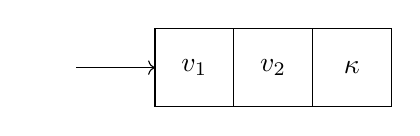
\begin{tikzpicture}[yscale=-1]
  \node at (0.5,0.5) {$\loc$} ;
  \draw [->] (1,0.5) -- ++(1,0) ;
  \draw (2,0) grid ++(3,1) ;
  \node at (2.5,0.5) {$v_1$} ;
  \node at (3.5,0.5) {$v_2$} ;
  \node at (4.5,0.5) {$\kappa$} ;
\end{tikzpicture}
\end{frame}

\begin{frame}{Finished MCAS}
\centering
\Large
\begin{minipage}[t][0.6\textheight]{0.48\textwidth}
  \[
    \loc \iKcasPointsto v_1
  \]
  \vfill
  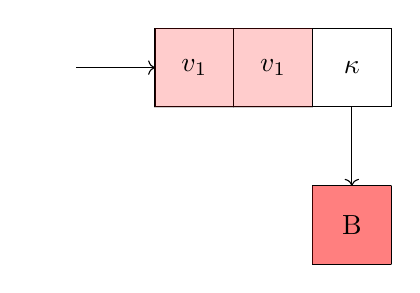
\begin{tikzpicture}[yscale=-1]
    \node at (0.5,0.5) {$\loc$} ;
    \draw [->] (1,0.5) -- ++(1,0) ;
    \draw (2,0) grid ++(3,1) ;
    \draw [fill=red, opacity=0.2] (2,0) rectangle ++(1,1) ;
    \node at (2.5,0.5) {$v_1$} ;
    \draw [fill=red, opacity=0.2] (3,0) rectangle ++(1,1) ;
    \node at (3.5,0.5) {$v_1$} ;
    \node at (4.5,0.5) {$\kappa$} ;
    \draw [->] (4.5,1) -- ++(0,1) ;
    \draw (4,2) grid ++(1,1) ;
    \draw [fill=red, opacity=0.5] (4,2) rectangle ++(1,1) ;
    \node at (4.5,2.5) {B} ;
  \end{tikzpicture}
\end{minipage}
\begin{minipage}[t][0.6\textheight]{0.48\textwidth}
  \[
    \loc \iKcasPointsto v_2
  \]
  \vfill
  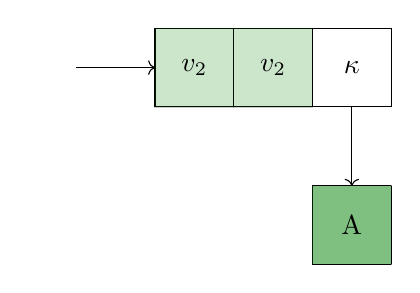
\begin{tikzpicture}[yscale=-1]
    \node at (0.5,0.5) {$\loc$} ;
    \draw [->] (1,0.5) -- ++(1,0) ;
    \draw (2,0) grid ++(3,1) ;
    \draw [fill=Green, opacity=0.2] (2,0) rectangle ++(1,1) ;
    \node at (2.5,0.5) {$v_2$} ;
    \draw [fill=Green, opacity=0.2] (3,0) rectangle ++(1,1) ;
    \node at (3.5,0.5) {$v_2$} ;
    \node at (4.5,0.5) {$\kappa$} ;
    \draw [->] (4.5,1) -- ++(0,1) ;
    \draw (4,2) grid ++(1,1) ;
    \draw [fill=Green, opacity=0.5] (4,2) rectangle ++(1,1) ;
    \node at (4.5,2.5) {A} ;
  \end{tikzpicture}
\end{minipage}
\end{frame}

\begin{frame}{Undetermined MCAS}
\centering
\Large
\[
  \loc \iKcasPointsto v_1
\]
\vfill
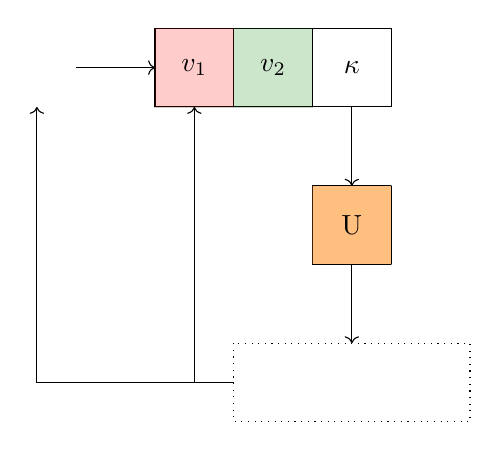
\begin{tikzpicture}[yscale=-1]
  \node at (0.5,0.5) {$\loc$} ;
  \draw [->] (1,0.5) -- ++(1,0) ;
  \draw (2,0) grid ++(3,1) ;
  \draw [fill=red, opacity=0.2] (2,0) rectangle ++(1,1) ;
  \node at (2.5,0.5) {$v_1$} ;
  \draw [fill=Green, opacity=0.2] (3,0) rectangle ++(1,1) ;
  \node at (3.5,0.5) {$v_2$} ;
  \node at (4.5,0.5) {$\kappa$} ;
  \draw [->] (4.5,1) -- ++(0,1) ;
  \draw (4,2) grid ++(1,1) ;
  \draw [fill=orange, opacity=0.5] (4,2) rectangle ++(1,1) ;
  \node at (4.5,2.5) {U} ;
  \draw [->] (4.5,3) -- ++(0,1) ;
  \draw [dotted] (3,4) rectangle ++(3,1) ;
  \draw [->] (3,4.5) -| (0.5,1) ;
  \draw [->] (3,4.5) -| (2.5,1) ;
\end{tikzpicture}
\end{frame}

\begin{frame}{MCAS algorithm}
\centering
\large
\begin{tikzpicture}[yscale=-1]
  \node at (0.5,0.5) {$\loc_1$} ;
  
  \draw (2,0) grid ++(3,1) ;
  \draw [fill=Green, opacity=0.2] (2,0) rectangle ++(1,1) ;
  \node at (2.5,0.5) {1} ;
  \draw [fill=Green, opacity=0.2] (3,0) rectangle ++(1,1) ;
  \node at (3.5,0.5) {1} ;
  \node at (4.5,0.5) {$\kappa_1$} ;
  \draw [->] (4.5,0) -- ++(0,-1) ;
  \draw (4,-2) grid ++(1,1) ;
  \draw [fill=Green, opacity=0.5] (4,-2) rectangle ++(1,1) ;
  \node at (4.5,-1.5) {A} ;
  
  \node at (7.5,0.5) {$\loc_2$} ;
  
  \draw (9,0) grid ++(3,1) ;
  \draw [fill=Green, opacity=0.2] (9,0) rectangle ++(1,1) ;
  \node at (9.5,0.5) {3} ;
  \draw [fill=Green, opacity=0.2] (10,0) rectangle ++(1,1) ;
  \node at (10.5,0.5) {3} ;
  \node at (11.5,0.5) {$\kappa_2$} ;
  \draw [->] (11.5,0) -- ++(0,-1) ;
  \draw (11,-2) grid ++(1,1) ;
  \draw [fill=Green, opacity=0.5] (11,-2) rectangle ++(1,1) ;
  \node at (11.5,-1.5) {A} ;
  
  \draw (2,2) grid ++(3,1) ;
  \only<1-4,7->{
    \draw [fill=red, opacity=0.2] (2,2) rectangle ++(1,1) ;
    \node at (2.5,2.5) {1} ;
  }
  \only<5-6>{
    \draw [fill=Green, opacity=0.2] (2,2) rectangle ++(1,1) ;
    \node at (2.5,2.5) {2} ;
  }
  \only<1-8>{
    \draw [fill=Green, opacity=0.2] (3,2) rectangle ++(1,1) ;
    \node at (3.5,2.5) {2} ;
  }
  \only<9->{
    \draw [fill=red, opacity=0.2] (3,2) rectangle ++(1,1) ;
    \node at (3.5,2.5) {1} ;
  }
  \node at (4.5,2.5) {$\kappa$} ;
  
  \draw (9,2) grid ++(3,1) ;
  \only<1-5>{
    \draw [fill=red, opacity=0.2] (9,2) rectangle ++(1,1) ;
    \node at (9.5,2.5) {3} ;
  }
  \only<6>{
    \draw [fill=Green, opacity=0.2] (9,2) rectangle ++(1,1) ;
    \node at (9.5,2.5) {2} ;
  }
  \only<7->{
    \draw [fill=red, opacity=0.2] (9,2) rectangle ++(1,1) ;
    \node at (9.5,2.5) {0} ;
  }
  \only<1-9>{
    \draw [fill=Green, opacity=0.2] (10,2) rectangle ++(1,1) ;
    \node at (10.5,2.5) {2} ;
  }
  \only<10->{
    \draw [fill=red, opacity=0.2] (10,2) rectangle ++(1,1) ;
    \node at (10.5,2.5) {0} ;
  }
  \node at (11.5,2.5) {$\kappa$} ;
  
  \only<1-3,7>{
    \draw [fill=orange, opacity=0.5] (7,4) rectangle ++(1,1) ;
    \node at (7.5,4.5) {U} ;
  }
  \only<4-6>{
    \draw [fill=Green, opacity=0.5] (7,4) rectangle ++(1,1) ;
    \node at (7.5,4.5) {A} ;
  }
  \only<8->{
    \draw [fill=red, opacity=0.5] (7,4) rectangle ++(1,1) ;
    \node at (7.5,4.5) {B} ;
  }
  
  \draw [->] (4.5,3) |- (7,4.5) ;
  \draw [->] (11.5,3) |- (8,4.5) ;
  
  \only<1>{
    \draw [->] (1,0.5) -- ++(1,0) ;
  }
  \only<2,7>{
    \draw [->, orange] (0.5,1) |- (2,2.5) ;
  }
  \only<3-6,8->{
    \draw [->] (0.5,1) |- (2,2.5) ;
  }
  
  \only<1-2,7->{
    \draw [->] (8,0.5) -- ++(1,0) ;
  }
  \only<3>{
    \draw [->, orange] (7.5,1) |- (9,2.5) ;
  }
  \only<4-6>{
    \draw [->] (7.5,1) |- (9,2.5) ;
  }
\end{tikzpicture}
\end{frame}

\section{Future work}

\begin{frame}{Coupling with semi-automated verification (\Gospel)}
\centering
\includegraphics[scale=0.6]{images/chargueraud_filliatre_lourenco_pereira.pdf}
\end{frame}

% ---------------------------------------------------------

\begin{frame}[plain, noframenumbering]
\centering
\huge
Thank you for your attention!
\end{frame}

% ---------------------------------------------------------

\end{document}
